% Created 2018-02-01 Thu 11:19
% Intended LaTeX compiler: pdflatex
\documentclass[10pt]{beamer}
\usepackage[utf8]{inputenc}
\usepackage[T1]{fontenc}
\usepackage{graphicx}
\usepackage{grffile}
\usepackage{longtable}
\usepackage{wrapfig}
\usepackage{rotating}
\usepackage[normalem]{ulem}
\usepackage{amsmath}
\usepackage{textcomp}
\usepackage{amssymb}
\usepackage{capt-of}
\usepackage{hyperref}
\logo{
\includegraphics[height=1.4cm,width=1.5cm]{RedHat-IsoLogo.jpg}}
\subtitle{Because we like silly names}
\institute{Red Hat}
\setbeamertemplate{navigation symbols}[horizontal]
\usepackage{pxfonts}
\usepackage{hyperref}
\hypersetup{colorlinks=true, linkcolor=red, filecolor=magenta, urlcolor=cyan}
\urlstyle{same}
\usepackage{minted}
\usepackage[utf8]{inputenc}
\usepackage[english]{babel}
\setbeamertemplate{caption}[numbered]
\setbeamercovered{invisible}
\usetheme{Frankfurt}
\usecolortheme{}
\usefonttheme{serif}
\useinnertheme{rounded}
\useoutertheme{}
\author{Sachin}
\date{\today}
\title{git}
\usecolortheme[RGB={0,104,139}]{structure}%deepskyblue
\hypersetup{
 pdfauthor={Sachin},
 pdftitle={git},
 pdfkeywords={git, version control},
 pdfsubject={Sample org beamer presentation},
 pdfcreator={Emacs 25.1.1 (Org mode 9.0.4)}, 
 pdflang={English}}
\begin{document}

\maketitle


\subsection{Intro}
\label{sec:org9656fa7}
\begin{frame}[label={sec:org3e2e206}]{What is git?}
\begin{quote}
A programs that remembers the changes in your file(s)
\end{quote}
\end{frame}

\begin{frame}[fragile,label={sec:org0797f98}]{Other version control systems}
 \begin{itemize}
\item Mercurial(\texttt{hg})
\item Subversion Control(\texttt{svn})
\item bazaar(\texttt{bzr})
\end{itemize}
\end{frame}

\subsection{Summary}
\label{sec:orgccbdb4f}
\begin{frame}[label={sec:orgf2be779}]{Why should I use git?}
\begin{itemize}
\item Once you get familiar it will be a part of you life.
\item Cleaner approach to file management
\end{itemize}
\end{frame}

\begin{frame}[label={sec:orga540567}]{Usefulness}
\begin{quote}
I'm no coder or a developer, can I use \alert{git}?
\end{quote}
\end{frame}


\begin{frame}[label={sec:org6343acc}]{Basic concept}
\begin{figure}[htbp]
\centering
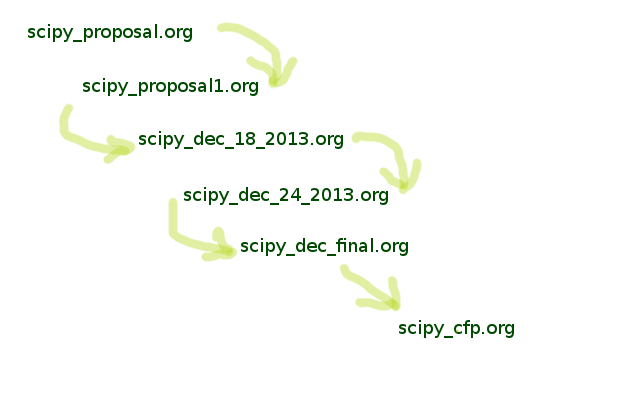
\includegraphics[width=.9\linewidth]{./concept.png}
\caption{\label{fig:org6cfa832}
life of a file}
\end{figure}
\end{frame}

\begin{frame}[fragile,label={sec:org44d3edb}]{Installing \texttt{git}}
 \begin{minted}[linenos,firstnumber=1]{sh}
# RHEL/Fedora
sudo dnf install git
# or
sudo yum install git

# Ubuntu
sudo apt-get install git
\end{minted}
\end{frame}


\begin{frame}[fragile,label={sec:org753a809}]{Basic setup}
 \begin{minted}[linenos,firstnumber=1]{sh}
# Your name
git config --global user.name "Sachin"

# Your Email
git config --global user.email "psachin@redhat.com"
\end{minted}
\end{frame}


\begin{frame}[fragile,label={sec:org26537d0}]{Create a project}
 \begin{minted}[linenos,firstnumber=1]{sh}
git init octo

# Check status of project
cd octo
git status
\end{minted}
\end{frame}

\begin{frame}[fragile,label={sec:orgb4439d0}]{Add file to the project}
 \begin{minted}[linenos,firstnumber=1]{sh}
# Create file
echo "git -- a version control tool" > introduction.txt

# Add file
git add introduction.txt

# or add everything within current directory
git add .

# or add files using wild card entries
git add *.txt
\end{minted}
\end{frame}

\begin{frame}[fragile,label={sec:orgee60fa0}]{Check status of your project}
 \begin{minted}[]{sh}
git status
\end{minted}
\end{frame}

\begin{frame}[fragile,label={sec:org3823ffa}]{Commit if your are happy :D}
 \begin{minted}[]{sh}
git commit -m "My message"
\end{minted}
\end{frame}


\begin{frame}[fragile,label={sec:org3804c9f}]{Make changes to file}
 \begin{minted}[]{sh}
echo "I use it to manage project" >> introduction.txt
\end{minted}
\end{frame}

\begin{frame}[fragile,label={sec:org4bda706}]{See changes w.r.t last commit}
 \begin{minted}[linenos,firstnumber=1]{sh}
git diff
# or
git diff introduction.txt
\end{minted}
\end{frame}


\begin{frame}[fragile,label={sec:org4236b8a}]{Update modified file(s)}
 \begin{minted}[linenos,firstnumber=1]{sh}
# to update already committed file
git add -u
\end{minted}

(\emph{do some more commits})
\end{frame}

\subsection{Log}
\label{sec:org06e84c7}
\begin{frame}[fragile,label={sec:org26d365d}]{View commits}
 \begin{minted}[]{sh}
git log

# Each commit on single line
git log --oneline

# A more decorated view. Looks great when working with branch
git log --graph --decorate --oneline
\end{minted}
\end{frame}

\section{GitHub}
\label{sec:org6b52598}
\subsection{Hosting your code}
\label{sec:org1adde17}

\begin{center}

\includegraphics[width=.9\linewidth]{./github.png}
\end{center}

\subsection{Branch}
\label{sec:orgef91365}
\begin{frame}[label={sec:org77a22a4}]{Git branch?}
\begin{center}
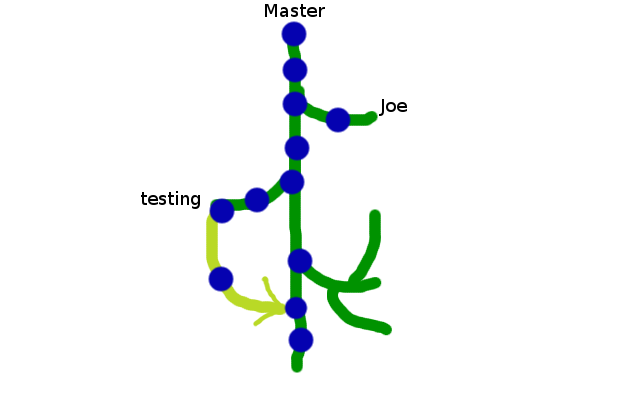
\includegraphics[width=.9\linewidth]{./branch.png}
\end{center}
\end{frame}

\begin{frame}[fragile,label={sec:org2fe5ce7}]{Git branch}
 \begin{minted}[linenos,firstnumber=1]{sh}
# Create new branch from master
git branch new-feature

# Change from master branch to new-feature branch
git checkout new-feature

# Or perform above steps in one go
git checkout -b new-feature
\end{minted}
\end{frame}

\begin{frame}[label={sec:org5798f2d}]{Git remote}
\begin{center}
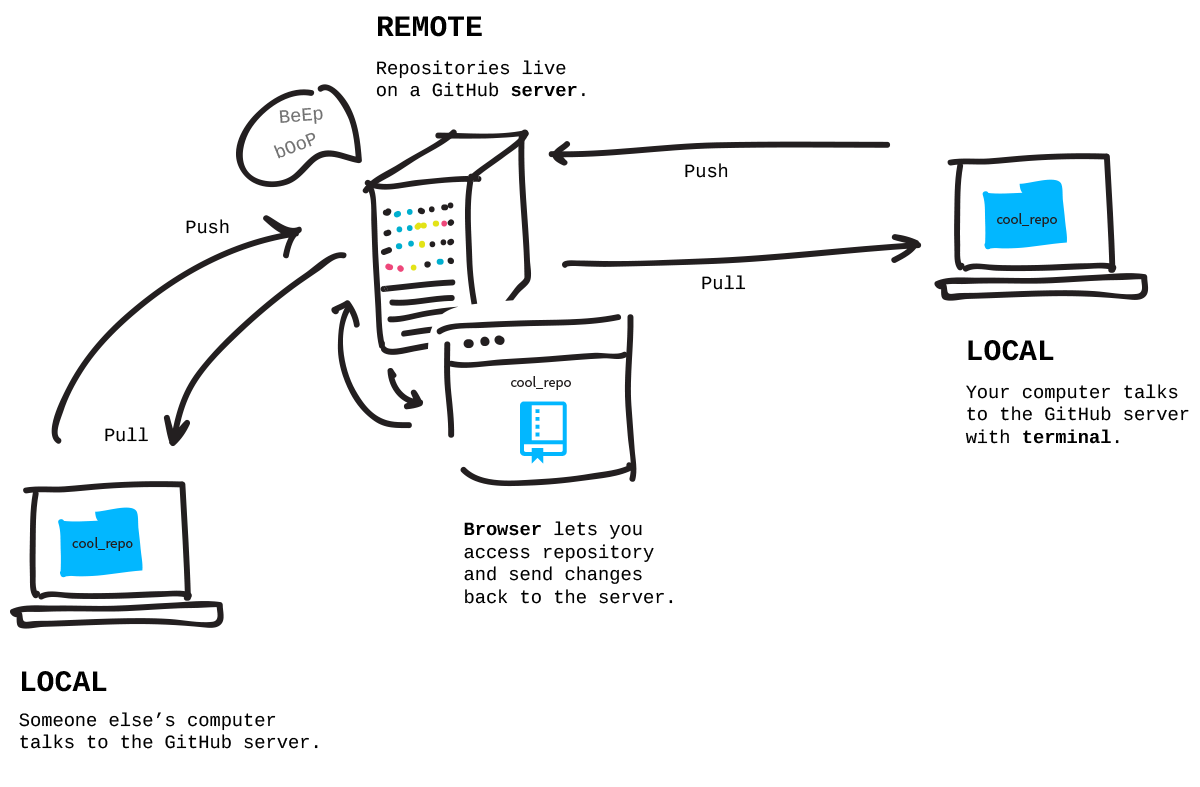
\includegraphics[width=.9\linewidth]{./remotes.png}
\end{center}

Image source: \url{http://jlord.us/git-it/challenges/remote\_control.html}
\end{frame}

\begin{frame}[fragile,label={sec:org6a01c72}]{Git remote}
 \begin{minted}[linenos,firstnumber=1]{sh}
# Display remote host
git remote
# Or add verbosity
git remote -v

# Syntax: Add remote hosts
git remote add <REMOTE_NAME> <REMOTE_URL>

# Example
git remote add origin https://github.com/psachin/octo.git
\end{minted}
\end{frame}

\begin{frame}[fragile,label={sec:org8236c74}]{git pull/push}
 \begin{minted}[linenos,firstnumber=1]{sh}
# Syntax: Push commit for the first time
git push -u <REMOTE_NAME <BRANCH_NAME>

# Example
git push -u origin master

# You can use 'git push' afterwards

# To download latest changes from current branch
# (assuming remote is added)
git pull
\end{minted}
\end{frame}

\subsection{Host}
\label{sec:orgb6f55a2}
\begin{frame}[label={sec:org46d9f1b}]{Hosting sites}
\begin{itemize}
\item savannah.gnu.org
\item gitlab.com
\item github.com
\item bitbucket.org
\item sourceforge.net
\item notabug.org
\end{itemize}
\end{frame}

\begin{frame}[label={sec:org0915c98}]{Thanks}
\begin{block}{git}
\url{https://git-scm.com/book/en/v2}
\end{block}
\end{frame}

\begin{frame}[label={sec:orgdbbcd57}]{Thanks}
\begin{block}{Email}
psachin@redhat.com
\end{block}
\begin{block}{IRC}
psachin@\{freenode, gnome, OFTC\}
\end{block}
\begin{block}{Blog}
\url{https://psachin.github.io}
\end{block}
\end{frame}
\end{document}
